%Lezione 2 i minuti si riferiranno a quelli visibili su teams e non quelli del file registrato con OBS
\subsection{Determinazione equazioni di stato di un circuito qualsiasi}

Si riprende la classe di circuiti lineari tempo invarianti (LTI), si suppone di conoscere
le variabili di stato $i_L(t) $ e $v_C(t) $ assumendole note, si sostituisce ogni \textit{condensatore}
con un generatore di tensione di valore pari alla $v_C(t)$, ripetendo il procedimento
per ciascun \textit{induttore} che viene sostituito con un generatore di corrente con corrente impressa
pari ad $i_L(t)$.

In queste condizioni, la soluzione del circuito resta formalmente invariata, 
il nuovo circuito sarà di tipo adinamico, non presenterà più alcun componente dinamico,
prende il nome di \textit{circuito resistivo associato al circuito di partenza}.

Il vantaggio di questa operazione è la possibilità di ricavare $v_L$ e $i_C$ utilizzando il principio
di \textit{sovrapposizione degli effetti} (PSE).

Si ricavano le equazioni di stato per il seguente circuito:
\begin{figure}[H]
\centering
\begin{circuitikz}
\draw
(0,0) to [voltage source,invert,l=$E$] (0,2)
to [R=$R_1$] (2,2)
to [C,v^=$v_C$,l_=$C$,i_=$i_C$] (2,0) -- (0,0)
;\draw
(2,2) to [R=$R_2$] (4,2)
to [L=$L$,i=$i_L$,v=$v_L$] (4,0) -- (2,0)
;
\end{circuitikz}
\end{figure}

Si applica il PSE, per trovare $i_C$ e $v_L$:
$$\begin{aligned}
i_C &= i_c' + i_C'' + i_C'''\\
v_L &= v_L' + v_L'' + v_L'''
\end{aligned}$$

\begin{figure}[H]
\centering
\begin{subfigure}{.49\linewidth} %Circuito C'
\centering
\begin{circuitikz}
\draw
(0,0) to [voltage source,invert,l=$E$] (0,2)
to [R=$R_1$] (2,2)
to [short,i_=$i_C'$] (2,0) -- (0,0)
;\draw
(2,2) to [R=$R_2$] (4,2)
to [open,v=$v_L'$] (4,0) -- (2,0)
;
\end{circuitikz}
\caption{Circuito 1}
\end{subfigure}
\begin{subfigure}{.49\linewidth} %Circuito C''
\centering
\begin{circuitikz}
\draw
(0,0) to [short] (0,2)
to [R=$R_1$] (2,2)
to [voltage source,v^=$v_C$,i>_=$i_C''$] (2,0) -- (0,0)
;\draw
(2,2) to [R=$R_2$] (4,2)
to [open,v=$v_L''$] (4,0) -- (2,0)
;
\end{circuitikz}
\caption{Circuito 2}
\end{subfigure}
\begin{subfigure}{.49\linewidth} %Circuito C'''
\centering
\begin{circuitikz}
\draw
(0,0) to [short] (0,2)
to [R=$R_1$] (2,2)
to [short,i_=$i_C'''$] (2,0) -- (0,0)
;\draw
(2,2) to [R=$R_2$] (4,2)
to [current source,i_=$i_L$,v^>=$v_L'''$] (4,0) -- (2,0)
;
\end{circuitikz}
\caption{Circuito 3}
\end{subfigure}
\end{figure}
\newpage
\begin{itemize}
\item Circuito 1)
$$
v_L' = 0;\ i_C' = \frac{E}{R_1} 
$$
\item Circuito 2)
$$
i_C'' = -\frac{v_C}{R_1};\ v_L'' = v_C
$$
\item Circuito 3)
$$
i_C''' = -i_L;\ v_L''' = -R_2\cdot i_L
$$
\end{itemize}
Sommando i tre contributi e aggiungendo il vincolo di continuità delle variabili
di stato si ottiene il problema di Cauchy del sistema:
$$\left\{\begin{aligned}
&i_C = \frac{E}{R_1} - \frac{v_C}{R_1} - i_L = C\frac{dv_C}{dt}\\
&v_L = v_C - R_2\cdot i_L = L\frac{di_L}{dt}\\
&i_L(0^+) = i_L(0^-)\\
&v_C(0^+) = v_C(0^-)
\end{aligned}\right.$$

\subsection{Circuiti lineari con generazioni impulsivi}
Si analizza ora un circuito che presenta generatori di tipo impulsivo, ad esempio la risposta di 
una linea elettrica a seguito di una fulminazione.
Si definisce quindi l'impulso rettangolare di ampiezza $\Delta$, la funzione viene chiamata 
$\Pi_\Delta(t)$, (funzione porta) è costante nell'intervallo $[-\frac{\Delta}{2},\frac{\Delta}{2}]$,
l'area del rettangoloide sotteso alla funzione è pari a
$$
\int_{-\Delta/2}^{\Delta/2}\Pi_\Delta(\tau)d\tau = 1\ \forall\ \Delta \in\ ]0,+\infty[
$$
Ha senso considerare la successione di funzioni ottenute per valori $\Delta$ decrescenti,
ma dimezzando la base, per mantenere l'area unitaria, va raddoppiata l'altezza.

Passando al limite per $\Delta \rightarrow 0^+$ la successione tende in maniera non ordinaria
ad un limite che non è una funzione ma può essere definita come funzione generalizzata,
ossia distribuzione, che prende il nome di \textbf{Delta di Dirac} ($\delta(t)$).

Proprietà della $\delta(t)$:
\begin{itemize}
\item È nulla $\forall\ t \neq 0$
\item Ha integrale unitario
\item Proprietà di campionamento $\int_{-\infty}^{+\infty}f(\tau)\delta(\tau-t_0)d\tau = f(t_0)$
\end{itemize}
\newpage
La proprietà di campionamento calcolata come l'integrale della $\delta(t_0)$ per una funzione ordinaria
permette di valutare la funzione ordinaria nel punto $t_0$ (pari a 0 in questo caso per semplicità)
in cui è centrata la $\delta(t_0)$, si dimostra
utilizzando la definizione di $\delta(t)$ mediante successioni di funzioni porta $\Pi_\Delta(t)$
$$
\int_{-\Delta/2}^{\Delta/2} f(\tau)\Pi_\Delta(\tau-t_0)d\tau = \frac{1}{\Delta} \int_{-\Delta/2}^{\Delta/2}  f(\tau)d\tau = \frac{1}{\Delta}f(\vartheta^*)\cdot\Delta= f(\vartheta^*)
$$
con $\vartheta^* \in\ \left]-\frac{\Delta}{2},\frac{\Delta}{2}\right[$. Eseguendo il limite $\Delta\to 0$ si ha
$\vartheta^* \to 0 $, in conclusione
$$
\int_{0^-}^{0^+} f(\tau)\delta(\tau)d\tau = f(0)
$$

Si analizza la funzione $U_\Delta(t)$ definita come segue:
\begin{equation*}
\begin{cases}
0 & t  < -\frac{\Delta}{2} \\
1 & t  > \frac{\Delta}{2} \\
\frac{1}{2}+\frac{t}{\Delta} & -\frac{\Delta}{2} \leq t \leq \frac{\Delta}{2}
\end{cases}
\end{equation*}
\begin{figure}[H]\centering
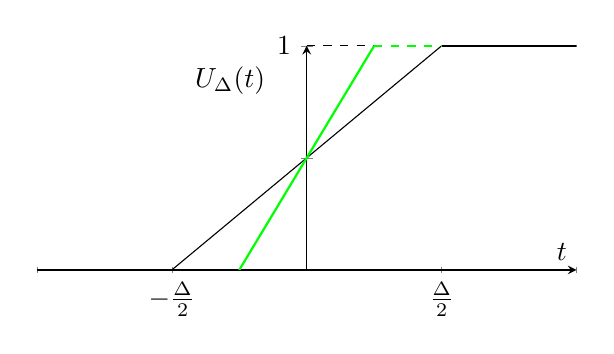
\begin{tikzpicture}
\begin{axis}[
    axis lines = center,
    xlabel = \(t\),
    ylabel = {\(U_\Delta(t)\)},
    ylabel style = {at={(axis cs: -0.9,0.95)}},
    xtick = {-2,-1,0,1,2},
    xticklabels = { , $-\frac{\Delta}{2}$, , $\frac{\Delta}{2}$,},
    ytick = {0 ,0.5 ,1},
    yticklabels = { , ,1},
    xmin =  -2, xmax = 2,
    yscale = 0.5,
]
%Below the red parabola is defined
\addplot [
    domain=-1:1, 
    samples=2, 
    color=black,
]
{0.5 + x/2};
\draw [thick] (axis cs:1,1) -- (axis cs:2,1);
\draw [thick] (axis cs:-2,0) -- (axis cs:-1,0);
\draw [dashed] (axis cs:0,1) -- (axis cs:0.5,1);
\addplot [
    domain = -0.5:0.5,
    samples = 2,
    color = green,
    style = thick,
]{0.5 + x};
\draw [thick,dashed,color = green] (axis cs:0.5,1) -- (axis cs:1,1);
\end{axis}
\end{tikzpicture}
\end{figure}

La derivata temporale nei punti regolari coincide quasi ovunque con la funzione $\Pi_\Delta(t)$.
Eseguendo il limite su $U_\Delta(t)$
di $\Delta \rightarrow 0^+$ come si nota dall'andamento del segmento in verde, si ottiene la funzione definita 
``gradino'' o funzione di Heaviside $u(t)$.
$$
u(t) = \begin{cases}
0 & t\leq 0\\
1 & t > 0
\end{cases}
$$


Un ulteriore modo per definire la $\delta(t)$ è appunto quella di derivata della funzione gradino $u(t)$.
$$
\delta(t) = \frac{d}{dt}u(t) \Leftrightarrow \int_{-\infty}^t \delta(\tau)d\tau = u(t)
$$
\newpage
\paragraph{Esempio con generatore impulsivo}
Si consideri un circuito RC serie
\begin{figure}[H]\centering
\begin{circuitikz}
\draw
(0,0) to [voltage source,invert,l=$e(t)$] (0,2)
      to [R=$R$] (2,2)
      to [C,l_=$C$,v^=$v_C$] (2,0) -- (0,0)
;
\end{circuitikz}
\end{figure}

una funzione 
$$
e(t) = \begin{cases}
E_0 & 0 < t < T\\
0 &\text{altrimenti}
\end{cases}
$$
Si vuole ricavare $v_C(t)$:

Si suppone che la condizione iniziale, per $t < 0 $, ossia la tensione sul condensatore sia nulla.
$$\begin{aligned}
&\begin{cases}
e(t) &= RC\frac{dv_C}{dt} + v_C \\
v_C(0) &= \SI{0}{\volt}
\end{cases}\\
&0 \leq t \leq T\\
&\begin{cases}
E_0 &= RC\frac{dv_C}{dt} + v_C \\
v_C^{(1)}(0) &= \SI{0}{\volt} 
\end{cases}\\
&t > T\\
&\begin{cases}
0 &= RC\frac{dv_C}{dt} + v_C \\
v_C^{(2)}(0) &= v_C^{(1)}(T) 
\end{cases}
\end{aligned}
$$
Conoscendo la forma della soluzione vanno solo sostituiti i termini nelle varie configurazioni
$$
v_C^{(1)}(t) = -E_0 e^{-\frac{t}{\tau}} + E_0,\ v_C^{(1)}(T) = E_0 \left(1-e^{-\frac{T}{\tau}}\right),\ \tau = RC
$$
$$
v_C^{(2)}(t) = E_0\left(1-e^{-\frac{T}{\tau}}\right) e^{-\frac{t-T}{\tau}} = v_C^{(1)}(T)\cdot e^{-\frac{t-T}{\tau}}
$$
In conclusione
$$
v_C(t) = \left\{
\begin{aligned}
&0 \qquad\qquad\qquad\qquad\qquad\ t\leq 0\\
&E_0 \left(1-e^{-\frac{T}{\tau}}\right) \qquad\qquad\ \ 0 < t < T\\
& E_0\left(1-e^{-\frac{T}{\tau}}\right) e^{-\frac{t-T}{\tau}} \qquad t \geq T
\end{aligned}\right.
$$
\begin{figure}[H]
\centering
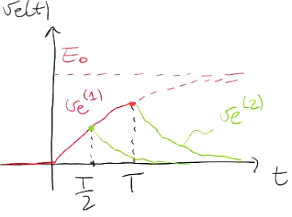
\includegraphics[width = 0.4\linewidth]{v_C_lezione_2}
\end{figure}

Si ottiene una funzione esponenziale crescente fino a $T$ e poi decrescente fino a 0 all'infinito. 
Diminuendo il valore di $T$ si vede che il ``picco'' della funzione sarà più basso, al limite 
di $T \rightarrow 0$ la soluzione si annulla.
Se si impone il prodotto $E_0\cdot T = 1$ ossia $E_0 = \frac{1}{T}$ e si esegue il limite invece:
$$
\lim_{T\rightarrow0^+} v_C(t)
$$
Il limite viene eseguito sulle singole parti della funzione, ad esempio nel tratto $0\leq t \leq T$
la funzione ha sempre un tempo inferiore per raggiungere il valore massimo, mentre l'ampiezza
del generatore aumenta.

Si suppone di sviluppare la funzione esponenziale con la sua serie di Taylor:
$$
e^x = 1 + x + \frac{x^2}{2!} + \frac{x^3}{3!} + ...\simeq 1 + x \Rightarrow 1-e^{-\frac{t}{\tau}} \simeq \frac{t}{\tau} 
$$
L'equazione della tensione diventa
$$v_C(t) = 
\begin{cases}
0\ & t\leq 0 \\
\frac{1}{T}\frac{t}{\tau}\  & 0 \leq t\leq T \\
\frac{1}{T}\frac{T}{\tau} e^{-\frac{t-T}{\tau}}\ & t\geq T
\end{cases}
$$
Per $T\rightarrow 0^+$
$$v_C(t) =
\begin{cases}
0\ & t\leq 0\\
\frac{1}{\tau}e^{\frac{-t}{\tau}}\ & t \geq 0
\end{cases}
$$

Il primo tratto dell'equazione si approssima quindi ad un tratto lineare fino a T, arrivando ad 
un'altezza di $\frac{1}{\tau}$, al limite raggiunge questo valore in un tempo infinitesimo.
\begin{figure}[H]
\centering
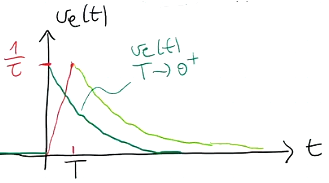
\includegraphics[width = 0.4\linewidth]{v_C_limite_lezione_2}
\end{figure}
Si otterrebbe la stessa soluzione ponendo $e(t) = \Pi_\Delta(t)$ e svolgendo il limite
$$\Pi_\Delta(t) \stackrel{\Delta\rightarrow0^+}{\rightarrow} \delta(t) \Rightarrow v_C(t) \rightarrow h(t)$$
$h(t)$ è chiamata risposta all'impulso del circuito dinamico.

In alternativa è possibile utilizzare direttamente un generatore impulsivo e risolvere il circuito

\begin{figure}[H]\centering
\begin{circuitikz}
\draw
(0,0) to [voltage source,invert,l=$\delta(t)$] (0,2)
      to [R=$R$] (2,2)
      to [C,l_=$C$,v^=$v_C$,i_=$i_C$] (2,0) -- (0,0)
;
\end{circuitikz}
\end{figure}

$$
\delta(t) = RC\frac{dv_C}{dt} + v_C \Rightarrow i_C = \frac{\delta(t)-v_C}{R}
$$
Se la tensione del generatore è impulsiva anche la corrente nel condensatore sarà di tipo impulsivo
mentre la tensione ai capi del condensatore si può ricavare integrando la sua equazione caratteristica
$$
i_c = C\frac{dv_C}{dt} \Rightarrow \int_{0^-}^{0^+} i_C(\tau)d\tau = C[v_C(0^+)-v_C(0^-)]
$$
$$
v_C(0^+) - v_C(0^-) = v_C(0^+) = \frac{1}{RC} \int_{0^-}^{0^+} \delta(\tau)d\tau - \cancel{\frac{1}{RC} \int_{0^-}^{0^+} v_C(\tau)d\tau} = 
$$
$$
= \frac{1}{RC} = \frac{1}{\tau}  \Rightarrow v_C(0^+) = \frac{1}{RC} = \frac{1}{\tau}
$$
Il secondo integrale vale zero perché esteso ad un intervallo infinitesimo di una funzione limitata,
perché legata all'energia immagazzinata nel condensatore che non può essere infinita.
% CONSIDERAZIONE PERSONALE
%dunque non potrebbe essere infinita a meno
%di non supporre un generatore dotato di potenza infinita (non possibile in questo caso data la 
%resistenza inserita nel circuito).
%
È infinita invece la potenza assorbita dal condensatore nell'istante $0^+$ che gli permette di avere
una tensione ai suoi capi discontinua.

\newpage
\subsection{Risposta al gradino unitario di un circuito dinamico LTI}
Stesso circuito del precedente, ma si utilizza come forzamento il gradino unitario di
Heaviside, la soluzione è più semplice della precedente:

$$
v_C(t) = \left(1-e^{-\frac{t}{\tau}}\right) u(t)
$$
viene chiamata $g(t)$ e si afferma che sia la risposta al gradino, ricordando la relazione
tra la funzione $\Pi_\Delta(t)$ e $U_\Delta(t)$ si ha che:
$$
\Pi_\Delta(t) = \frac{U_\Delta\left(t+\frac{\Delta}{2}\right)-U_\Delta\left(t-\frac{\Delta}{2}\right)}{\Delta} = e(t)
$$
per $\Delta \rightarrow 0^+$ si ottiene $h(t) = v_C(t)$ ossia la risposta all'impulso.

Essendo il circuito tempo invariante, si può trovare la risposta alla funzione $\Pi_\Delta(t)$
come combinazione lineare delle risposte delle due $U_\Delta$ opportunamente traslate, ossia
la risposta al gradino traslata.
$$
\text{Risp}\left\{ \Pi_\Delta(t)\right\} = \frac{\text{Risp}\left\{U_\Delta\left(t+\frac{\Delta}{2}\right)\right\} - 
\text{Risp}\left\{U_\Delta\left(t-\frac{\Delta}{2}\right)\right\}}{\Delta} = 
\frac{g\left(t+\frac{\Delta}{2}\right) - g\left(t-\frac{\Delta}{2}\right)}{\Delta}
$$
Tutto si trasforma nella funzione rapporto incrementale della funzione $g(t)$ ossia
$$
\lim_{\Delta\rightarrow0^+}\text{Risp}\left\{\Pi_\Delta(t)\right\} = h(t) = \frac{dg}{dt}
$$

$$
h(t) = \frac{dg}{dt} =\begin{cases}
0& t < 0\\
\frac{1}{\tau}e^{-\frac{t}{\tau}} & t\geq0 
\end{cases}
$$
La risposta all'impulso del circuito è quindi pari alla derivata della risposta al gradino dello stesso
circuito.
